\documentclass[twoside=false, DIV=14]{scrartcl}

\usepackage{arev} % order matters, putting this above allows FiraSans to override it for body text
\usepackage[sfdefault]{FiraSans}
\usepackage{inconsolata}
%\usepackage[fira]{fontsetup}
\usepackage{scrlayer-scrpage}
\renewcommand{\titlepagestyle}{scrheadings}
\usepackage{graphicx}
\usepackage{blindtext}
\usepackage{wrapfig}
\usepackage{tabularx}
\usepackage{hyperref}
\usepackage{listings}
\usepackage{tikz}
\usepackage{amsmath}
\usepackage[many]{tcolorbox}

\usepackage{xcolor,sectsty}
\definecolor{blackish}{RGB}{56,58,54}
\definecolor{redish}{RGB}{109,41,49}
\definecolor{red}{RGB}{152,41,50}
\definecolor{orangeish}{RGB}{188,71,0}
\definecolor{blueish}{RGB}{25,33,139}
\subsubsectionfont{\color{blackish}}
\subsectionfont{\color{blackish}}
\sectionfont{\color{blackish}}

\lohead{\color{red} COMP3000 Programming Languages}
\rohead{
\includegraphics[width=0.5cm]{../logo.jpg}}

\setkomafont{author}{\sffamily \small}
\setkomafont{date}{\sffamily \small}

\DeclareOldFontCommand{\bf}{\normalfont\bfseries}{\mathbf}
\DeclareOldFontCommand{\tt}{\normalfont\ttfamily}{\texttt}

\lstset{basicstyle=\ttfamily}


\date{}
\newtcolorbox{aside}[1][]{
  title=Aside,
  width=0.3\textwidth,
  fonttitle=\bfseries,
  breakable,
  fonttitle=\bfseries\color{black},
  colframe=blueish!80,
  colback=blueish!2
  #1}

\newtcolorbox{note}[1][]{
  title=Note,
  width=\textwidth,
  fonttitle=\bfseries,
  breakable,
  fonttitle=\bfseries\color{black},
  colframe=orangeish!80,
  colback=orangeish!2
  #1}

\newtcolorbox{hint}[1][]{
    title=Hint,
    width=\textwidth,
    fonttitle=\bfseries,
    breakable,
    fonttitle=\bfseries\color{white},
    colframe=blueish!80,
    colback=blueish!2
    #1}

\newtcolorbox{todo}[1][]{
  title=!! TODO !!,
  width=\textwidth,
  fonttitle=\bfseries,
  breakable,
  fonttitle=\bfseries\color{white},
  colframe=red!80,
  colback=red!2
  #1}
  
\providecommand{\tightlist}{%
  \setlength{\itemsep}{0pt}\setlength{\parskip}{0pt}}

\title{\color{redish} \vspace{-1em}COMP3000 Week 5: Abstract Syntax Trees and Grammars}

\begin{document}
{\color{blackish}\maketitle}\vspace{-7em}

\begin{abstract}
\end{abstract}

\section*{Topics}
\begin{enumerate}
\item Evaluation is Tree Traversal
\item Context Free Grammars
\item Intro to Metaprogramming
\end{enumerate}

\section*{Preparation}
\begin{itemize}
\item Read the text chapters X
\item Watch lectures, X
\item Complete the RAT individually and bring your answers to class.
\end{itemize}

\section*{Definitions to help while preparing}
\begin{description}
\item[Composition:] If you can process the parts, then combine them OR process the whole and still get the same result—you have something that \emph{composes}. This is a desirable property of any system.

\item[Metaprogramming:] Metaprogramming plays a big role this week, and this is the first time we have ever seen it. Metaprogramming is "a program that creates another program." In our case, a Java program is creating another Java program for us. If you think about it, we write a Java program, which we compile and run. When we run it, it creates another Java program (as source code). Now we have to compile and run that program! Other phrases for this idea include staged compilation, macro programming, or reflection—though there are subtle differences between those terms.

\end{description}

\newpage
\part*{RAT 5}
%\renewcommand{\labelenumii}{\alph{enumii}) $\fbox{$\phantom{x}$}$}
\renewcommand{\labelenumii}{\alph{enumii}) $\square$}
\begin{enumerate}
\item \textbf{question}
\begin{enumerate}
  \item answer \tick
  \item distractor
  \item distractor
  \item distractor
  \item distractor
\end{enumerate}
  \item \textbf{expression from tree four}
  Which lox expression corresponds to the following tree?
  
  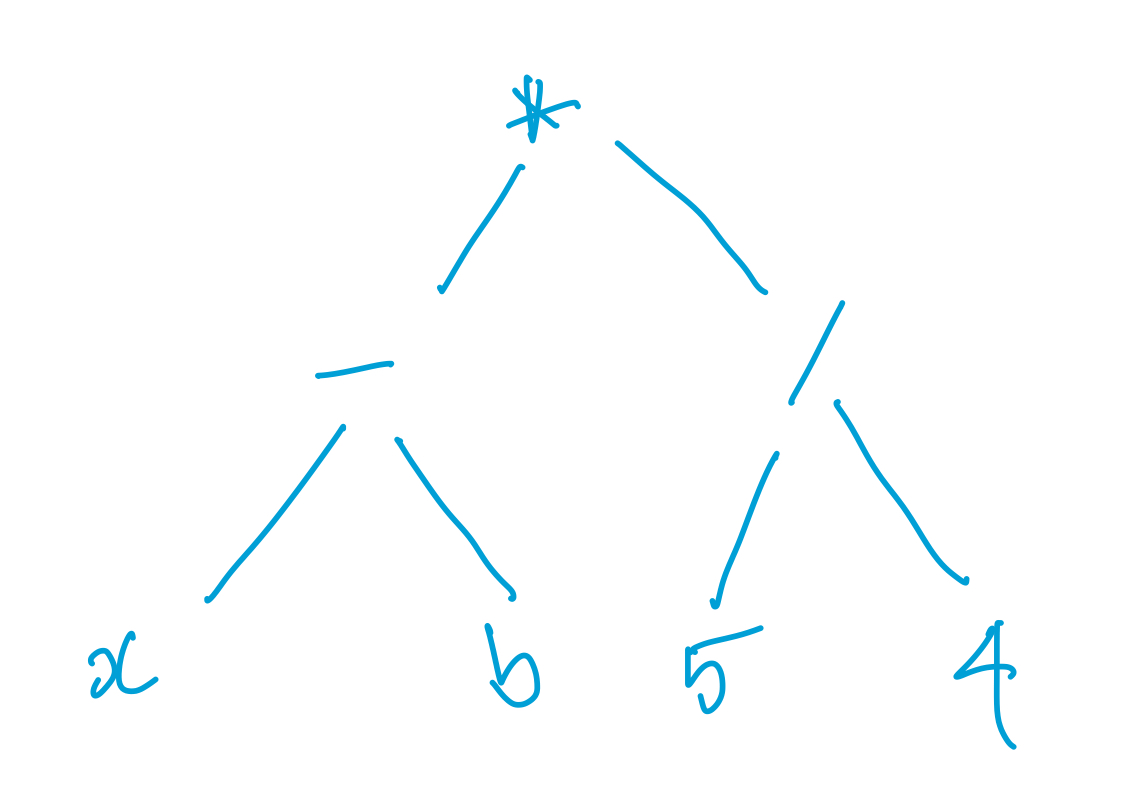
\includegraphics[width=\textwidth]{expr_tree_four.jpeg}
  
  There is only one correct answer, don't include any spaces in your answer so your answer will match and be graded accurately.  Note: the answer is a valid lox program, i.e. a string.%{=(x-b)\*(5/4) =(x-b)\*(5/4);}
  \begin{todo}
  The answers are commented out in the source, make distractors and turn all these into multiple choice questions
  \end{todo}

  \item \textbf{expression from tree two}
  Which lox expression corresponds to the following tree? 
  
  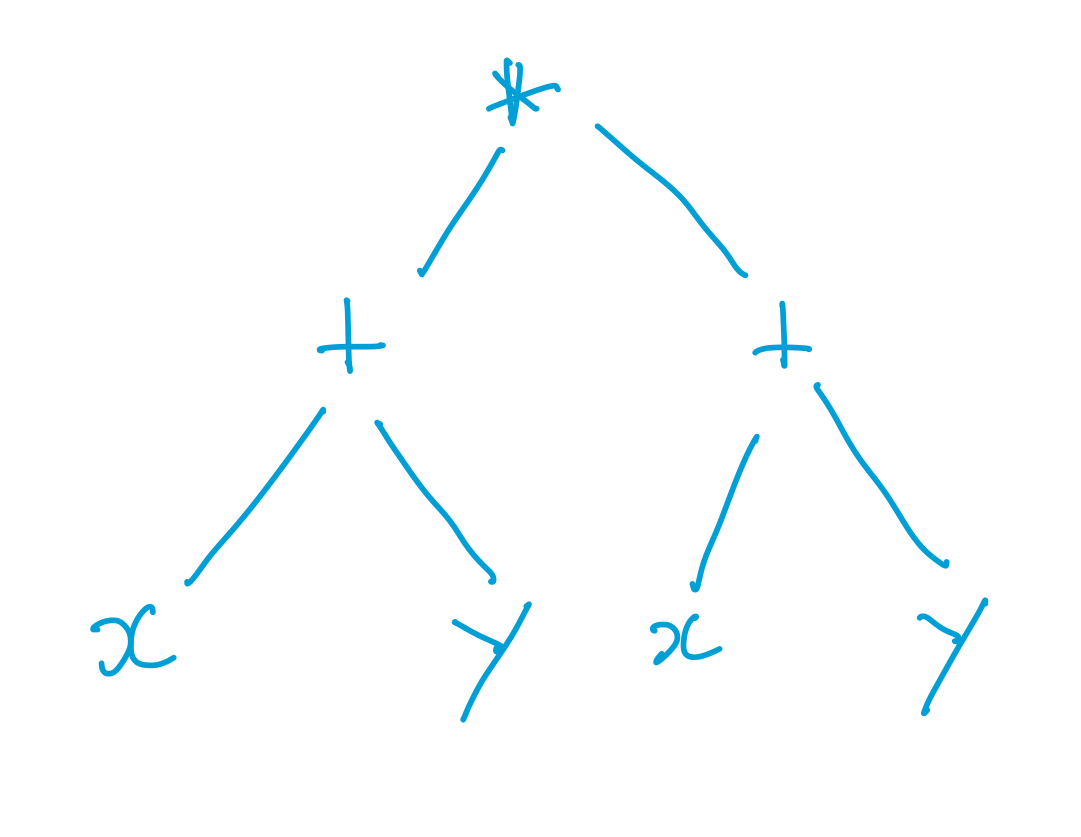
\includegraphics[width=\textwidth]{expr_tree_two.jpeg}
  
  There is only one correct answer, don't include any spaces in your answer so your answer will match and be graded accurately.  Note: the answer is a valid lox program, i.e. a string.%{=(x+y)\*(x+y) =(x+y)\*(x+y);}
  
  \item \textbf{expression from tree three}
  Which lox expression corresponds to the following tree? 
  
  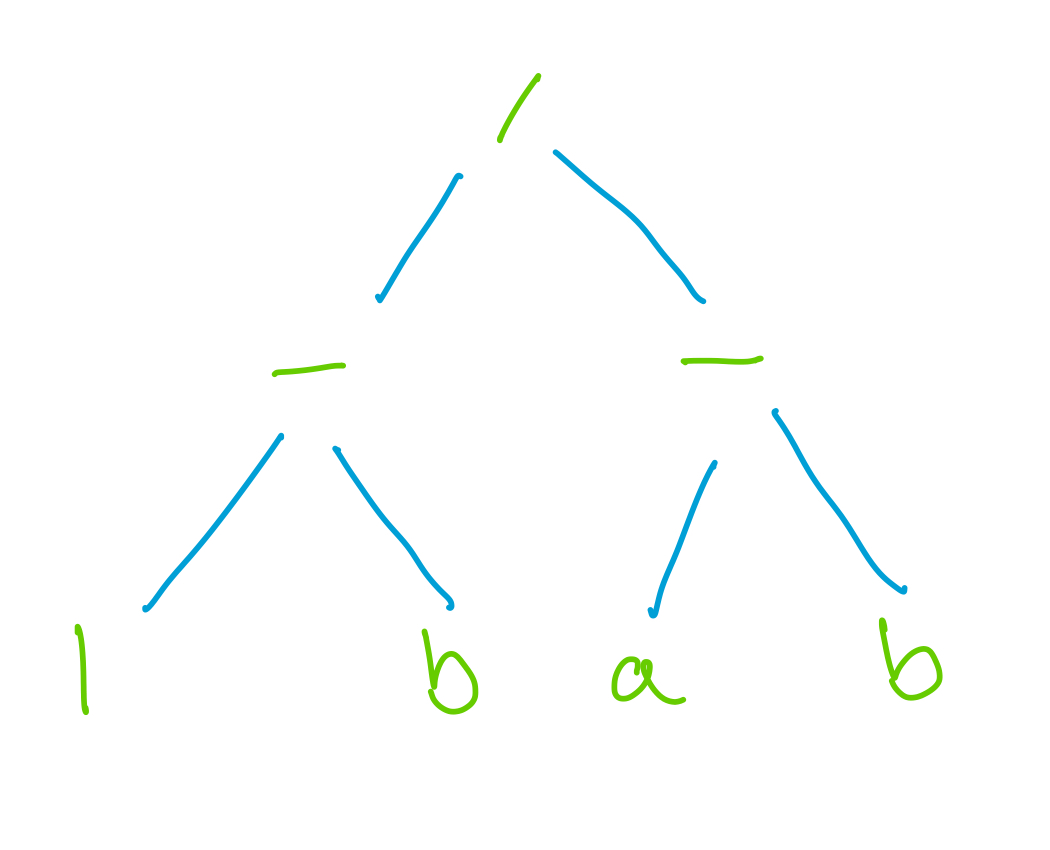
\includegraphics[width=\textwidth]{expr_tree_three.jpeg}  
  
  There is only one correct answer, don't include any spaces in your answer so your answer will match and be graded accurately.  Note: the answer is a valid lox program, i.e. a string.%{=(1-b)/(a-b) =(1-b)/(a-b);}
  

  \item \textbf{terminals}
  In the following grammar, which symbols are "terminals"
  \begin{lstlisting}
  e -> t | f ;
  t -> "foo" | "bar" ;
  f -> "foo()" | "bar()" ;
  \end{lstlisting}
  \begin{enumerate}
    \item e, t, and f
    \item e and t
    \item "foo" and "bar"
    \item \tick "foo", "bar", "foo()", and "bar()"
  \end{enumerate}
  
\item \textbf{lexemes}
Terminals are represented with a quoted string in the \emph{metasyntax}.  Which of the concepts we've seen so far represent terminals in our interpreter?
\begin{enumerate}
    \item \tick Tokens
    \item Characters
    \item Strings
    \item Trees
    \item Interpreters
    \item Compilers
    \item Grammars
\end{enumerate}

\item \textbf{simple grammar generation}
Given the following grammar, which is a string that could be generated?
\begin{lstlisting}
a -> b | c ;
b -> "matt" d ;
c -> "damian" e ;
d -> "makes me sad" |  "broke my skateboard" | "ate my lunch" ;
e -> "is tops" | "is my favourite" ;
\end{lstlisting}
\begin{enumerate}
    \item "matt is tops"
    \item "damian broke my skateboard"
    \item \tick "damian is tops"
    \item "matt is damian"
    \item "damian is matt"
\end{enumerate}

\end{enumerate}

\newpage
\part*{Application Exercise}

The Murray Darling Basin Authority (MDBA) is a government agency in Australia that manages the water resources of the Murray-Darling Basin. In this task you are going to write a little language to help the MDBA compute expected water flows.

Every river has a \emph{catchment} - all the land that drains into that river.  You are aware, I am sure, that rivers flow into other rivers son the border from one to another is not obvious \emph{on the ground} but decisions are made by the powers that be so that every drop of rain falls into a single catchment.  You can look up where each catchment is and which rivers flow into others in public geographic data if you like, but we will work from the ACT waterways to start with as shown in figure \ref{fig:act_waterways}.

Note that in this example, the final flow we are interested in is the flow out of Lake Burley Griffen (which is teh flow out of the Central Molongolo region).  This means you don't need to dealw tih teh left hand side of Figure \ref{fig:act_waterways} at all, we will come to that part in later weeks.

\begin{figure}
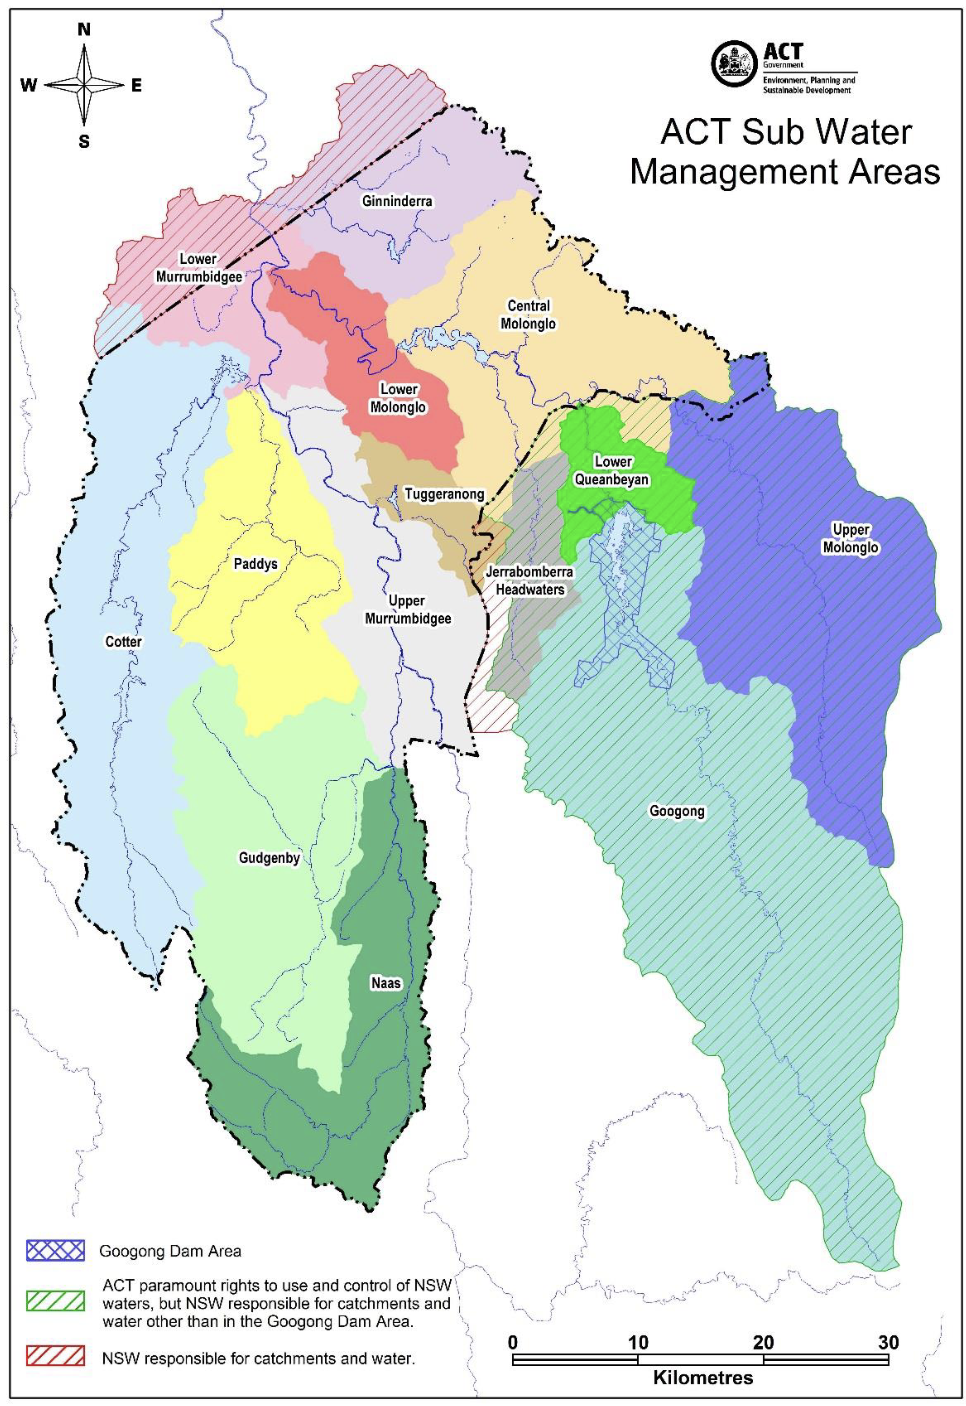
\includegraphics[width=\textwidth]{act_waterways.png}
\caption{Image source from the MDBA website}
\label{fig:act_waterways}
\end{figure}

Your job is to write an \emph{expression language} that can represent a flow in an arbitrary river and then to use that language to represent the flow out of Lake Burley Griffen.  The expression language should be able to represent the following things:

\begin{itemize}
  \item Some rivers are the start of a flow, these are the rivers that have no rivers flowing into them.  For example, the Cotter River is one such river.
  \item Other rivers are the result of a flow from one or more other rivers.  For example, the Upper Murrumbidgee River is the result of the flow from the Gudgenby River and the Naas River.
  \item The flow of a river is the sum of the flows of all the rivers that flow into it plus a new amount for its own catchment.  For example, the flow of the Upper Murrumbidgee River is the sum of the flow of the Gudgenby River and the Naas River plus some more from it's own catchement.\footnote{ There is a little fudge in this figure \ref{fig:act_waterways} which we will ignore.  The Upper Murrumbidgee actually starts a long way away and flows into the ACT at the southern end of the grey area but we will pretend it starts right at the boundary of the grey area so we have a workable task.  Once we build up more of our language, we can add in the rest of the Upper Murrumbidgee}.
  \item Dams act as a boundary for a catchment, even though there is only one up stream and one down stream flow.  The Dam will affect the flow in some way.
\end{itemize}

Draw the expression tree for the expression you have created.

\newpage
\part*{Application Exercise Notes and Solutions}
I came up with the following expression language:
\begin{lstlisting}
flow      -> [flow*] + additional  
          | headwater 
          | flow @ rate
          | "(" flow ")";
headwater  -> STRING;
rate       -> STRING;
additional -> STRING;
\end{lstlisting}

With this notation, I got:
\begin{lstlisting}
  ([UpperMolongolo, Googong @ Dam1 + LowerQueenbeyan, Jerrabomberra]
   + CentralMolongolo) @ Dam2
\end{lstlisting}

It makes way more sense to use numbers, but then you need to make up arbitray numbers.  I do suggest the students do that though which will result in somethingn like this:
\begin{lstlisting}
  ([3200, 5100 @ 50 + 800, 1050] + 2900) @ 90
\end{lstlisting}

\newpage
\part*{Self Study Exercises}
\section*{exercise}
flobadob

\subsection*{Solution}
dibdob


\section*{arithmetic as trees}
Consider the following arithmetic expression
\begin{lstlisting}
    2 / 3 + 3 + (8 * 3)
\end{lstlisting}
Draw a tree representation of the expression and evaluate it in the order you would do it in your head (following PEMDAS rules).  Label each part of the tree with a number indicating the order in which it would be evaluated.
\subsection*{Solution}
  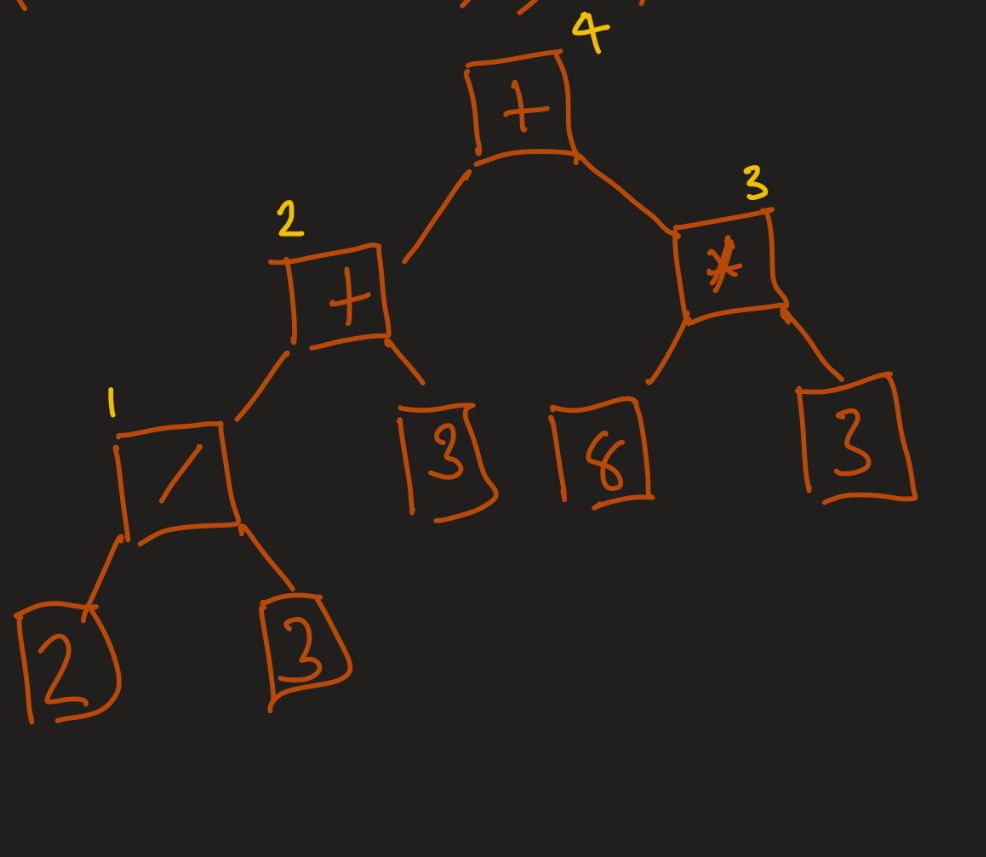
\includegraphics[width=\textwidth]{tree.jpeg}

\section*{trees as arithmetic}
  Write the expression corresponding to the following tree (do not include spaces in your answer):
  %\includegraphics[width=\textwidth]{expr-tree-cropped.png}
  \begin{todo}
  where is expression tree cropped?
  \end{todo}
\subsection*{Solution}
  \lstinline|(a+b)*c-(x-y)/z|

\section*{tree from expression}
  Using the paper you have been provided, draw the tree that should be generated from this expression according to PEMDAS rules.  This question is not asking about the Lox parser or any one grammar, it is asking about the rules we apply in arithmetic when evaluating this term.  You should draw some type of tree which represents the order of evaluation.  The expression in question is \lstinline|1 + 2 + 3 + 4|
\subsection*{Solution}
  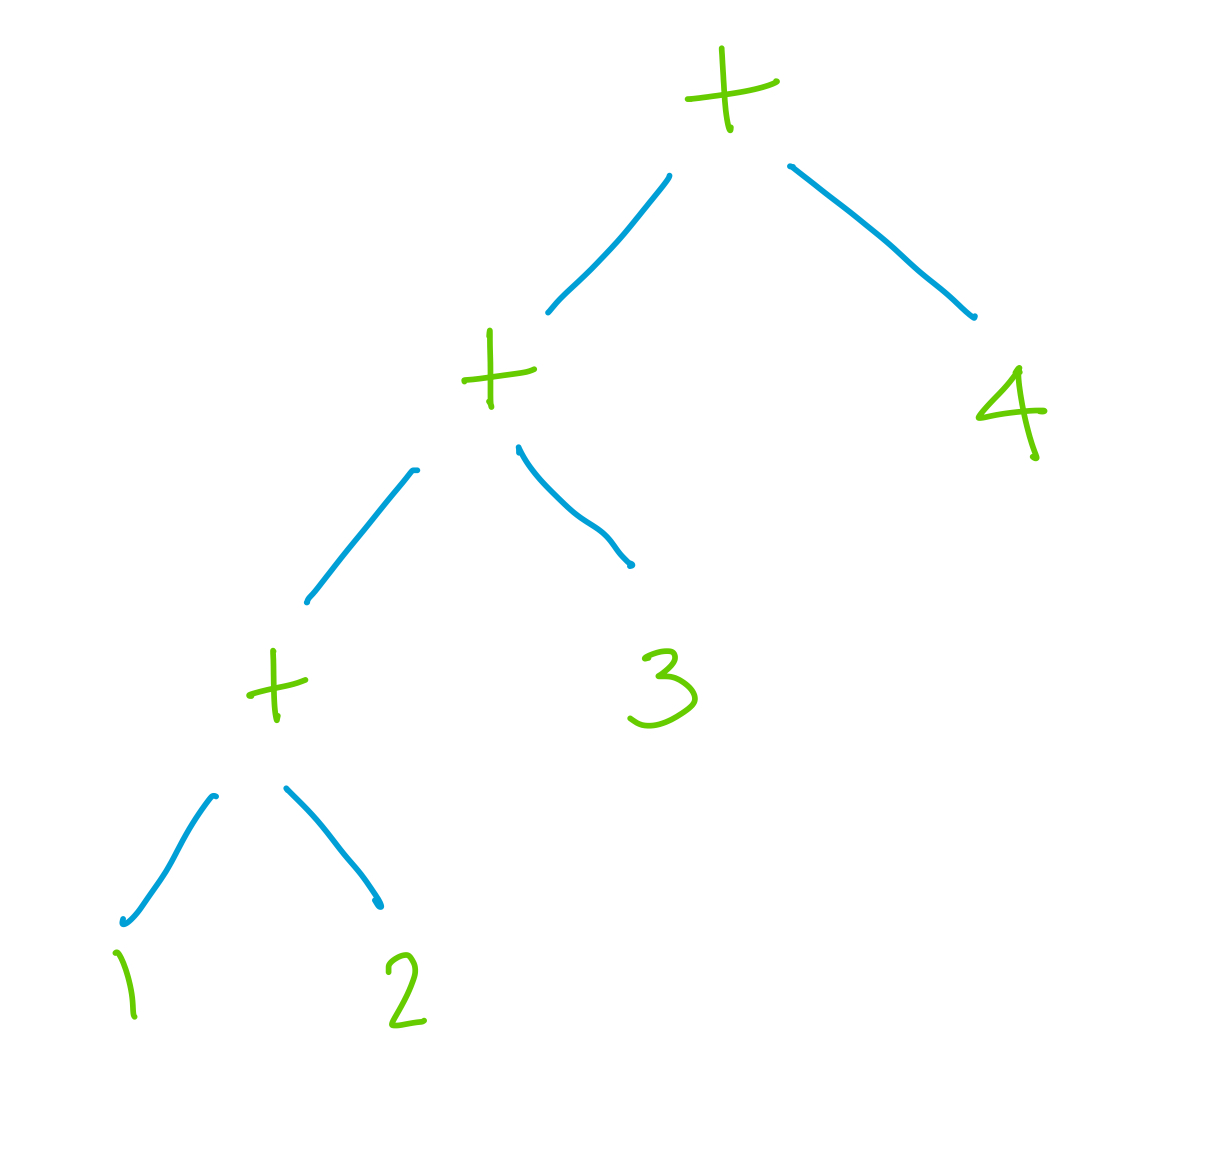
\includegraphics[width=\textwidth]{expr_tree_five.jpeg}


\section*{generate from grammar}
  Consider the following grammar
\begin{lstlisting}
  program -> statement* ;
  statement -> "print " expression "; " | "$" NUMBER " = " expression "; " ;
  expression -> NUMBER | STRING | expression " + " experssion | expression " && " expression |"$"NUMBER;
\end{lstlisting}

  Generate three sentances in this grammar that are at least 30 characters long. Can you generate any nonsensical sentances with this grammar?  Side note: using "\lstinline|$|" before variables is an old-school trick.
\subsection*{Solution}
  I generated the following
  \begin{itemize}
    \item \lstinline|"$1 = 5; print $1; $2=$1; print $1 + $2;"|
    \item \lstinline|"$12 = 5678 && 3456 + $1 && $2; print $33433 && $77"|
    \item \lstinline|"print 5; print 5; print 5; print 5; print 5; print 5;"|
  \end{itemize}
  I couldn't come up with something I thought was completely nonsensical, even if I found it hard to guess what some of the strings might mean.

\section*{arithmetic terminals}
  consider the arithmetic expression we did in the earlier question
\begin{lstlisting}
"  2 / 3 + 3 + (8 * 3)"
\end{lstlisting}  
If I told you this string was generated from a grammar:
\begin{itemize}
    \item would you believe me?
    \item what would the terminals in the grammar be?
    \item (optional) can you write out what you think the grammar was?
\end{itemize}
\subsection*{Solution}
  Yes of course, you wouldn't lie to me.  I think the terminals might be NUMBER, "+", "/", "*", "(", ")"
  I think the grammar might be
  \begin{lstlisting}
  A -> A "+" A | A "/" A | A "*" A | "(" A ")" | NUMBER
  \end{lstlisting}

\section*{write a context free grammar}
Write a context free grammar that can recognise strings according to the following rules. Use a notation similar to the one used in the book.
\begin{itemize}
    \item The string "wa " can appear as few as one time or as many as infite times
    \item The string "wa " can never appear anywhere besides the start or after another "wa "
    \item The string "nee " can only appear after a "wa" string
    \item The string " grey" can only appear as the last thing.
\end{itemize}
  Example strings are:
\begin{itemize}
    \item "wa wa wa wa nee  grey"
    \item "wa "
    \item "wa  grey"
    \item "wa nee  grey"
    \item "wa  grey"
    \item "wa wa "
\end{itemize}
\subsection*{Solution}
  This is a simple grammar in the end
  \begin{lstlisting}
  program = "wa "+ rem
  rem = ("" | "nee ") last
  last = ("" | " grey")
\end{lstlisting}

There are plenty of other valid grammars, but this is mine.

\section*{Writing a meta-program}
  There is quite a lot going on in this meta-programming idea.  To ensure we have it straight in our head, we will make our own metaprogrammer for a simple task.
  Write a Java program which will generate a "Hello world" Java program.  Once you have done that, parameterise that function so it can generate hello world programs that output different text.  Have it generate 3 programs, one which outputs \lstinline|"hello_world"|, another that outputs \lstinline|"gday_mate"| and a third that outputs \lstinline|"well_sod_ya_then"|.
\subsection*{Solution}
  Here is my program to create these programs.  I chose to put mine in a package called "meta" and that is where the generated programs will go to (but I will put them in a subpackage "generated").
  \lstinputlisting{HelloThere.java}



\end{document}